\documentclass[12pt]{report}
\usepackage[utf8]{inputenc}
\usepackage[myheadings]{fullpage}
\DeclareUnicodeCharacter{0301}{\hspace{-1ex}\'{ }}
% Package for headers 
\usepackage{fancyhdr}
\usepackage{lastpage}
\usepackage{longtable}

% For figures and stuff
\usepackage{graphicx, wrapfig, subcaption, setspace, booktabs}
\usepackage[T1]{fontenc}
\usepackage[export]{adjustbox}


% Change for different font sizes and families
\usepackage[font=small, labelfont=bf]{caption}
\usepackage{fourier}
\usepackage[protrusion=true, expansion=true]{microtype}

% Maths
\usepackage{amsmath,amssymb}
\usepackage{float}
\usepackage{graphicx}
\usepackage{wrapfig}
\usepackage[colorinlistoftodos]{todonotes}
\usepackage[colorlinks=true, allcolors=blue]{hyperref}

% Bibliography
\usepackage{biblatex}
\addbibresource{references.bib}

%% Language and font encodings
\usepackage[french]{babel}
\usepackage{csquotes}

\usepackage{multirow}

%% PDF
\usepackage{pdfpages}
%% Outlines
\usepackage{outlines}

% More styles for bullets
\usepackage{pifont}

\newcommand{\HRule}[1]{\rule{\linewidth}{#1}}
\renewcommand\footnoterule{\kern-3pt \hrule width 0.5\textwidth \kern 2.6pt}
\onehalfspacing
\setcounter{tocdepth}{5}
\setcounter{secnumdepth}{5}

%% Sets page size and margins
\usepackage[a4paper, margin=2.5cm]{geometry}
\linespread{1.15}
\usepackage{subfiles} % Best loaded last in the preamble

\usepackage[acronym]{glossaries}


\pagestyle{fancy}
\fancyhf{}

% Header and footer information
\setlength\headheight{15pt}
\fancyhead[L]{5TWIN2} 
\fancyhead[R]{Bilel Taktak}
\fancyfoot[R]{\thepage}
 \setlength {\marginparwidth }{2cm}

%acronyms%
\makeglossaries
\newacronym{it}{IT}{Information Technology}
\newacronym{ssr}{SSR}{Server Side Rendering}
\newacronym{ssg}{SSG}{Static Site Generation}
\newacronym{wip}{WIP}{Work in progress (Travail en cours)}
\newacronym{cicd}{CI/CD}{Continuous Integration and Continuous Delivery/Deployment (Intégration Continue et Développement/Livraison Cotinue)}
\newacronym{asss}{Amazon S3}{Amazon Simple Storage Service}
\newacronym{orm}{ORM}{Object Relational Mapping}
\newacronym{devops}{DevOps}{Development And Operations}
\newacronym{devsecops}{DevSecOps}{Development, Security, and Operations}
\newacronym{https}{HTTPS}{Hypertext Transfer Protocol Secure}
\newacronym{api}{API}{Application Programming Interface}
\newacronym{es}{ES}{ECMAScript}
\newacronym{es5}{ES5}{ECMAScript5}
\newacronym{es6}{ES6}{ECMAScript6}
\newacronym{es7}{ES7}{ECMAScript7}
\newacronym{ast}{AST}{Abstract Syntax Tree}
\newacronym{jit}{JIT}{Just-In-Time}
\newacronym{css}{CSS}{Cascading Style Sheets}
\newacronym{jsx}{JSX}{JavaScript XML}
\newacronym{js}{JS}{JavaScript}
\newacronym{sfc}{SFC}{Single-File Components}
\newacronym{json}{JSON}{JavaScript Object Notation}
\newacronym{jee}{JEE}{Java Enterprise Edition}
\newacronym{ui}{UI}{User Interface}
\newacronym{sql}{SQL}{Structured Query Language}
\newacronym{html}{HTML}{Hypertext Markup Language}
\newacronym{lts}{LTS}{Long Term Support}
\newacronym{ide}{IDE}{Integrated Development Environment}
\newacronym{sass}{Sass}{Syntactically Awesome Style Sheets}
\newacronym{pdf}{PDF}{Portable Document Format}
\newacronym{ai}{A.I}{Artificial Intelligence}

\renewcommand*{\glstextformat}[1]{\textbf{\color{black}#1}}
\hypersetup{citecolor=black}
\begin{document}
\clearpage\thispagestyle{empty}\addtocounter{page}{-1} 

\includepdf[pages=1, fitpaper=true]{pdf/Page_de_Garde_Ang_split_3.pdf}
\clearpage\thispagestyle{empty}\addtocounter{page}{-1} 
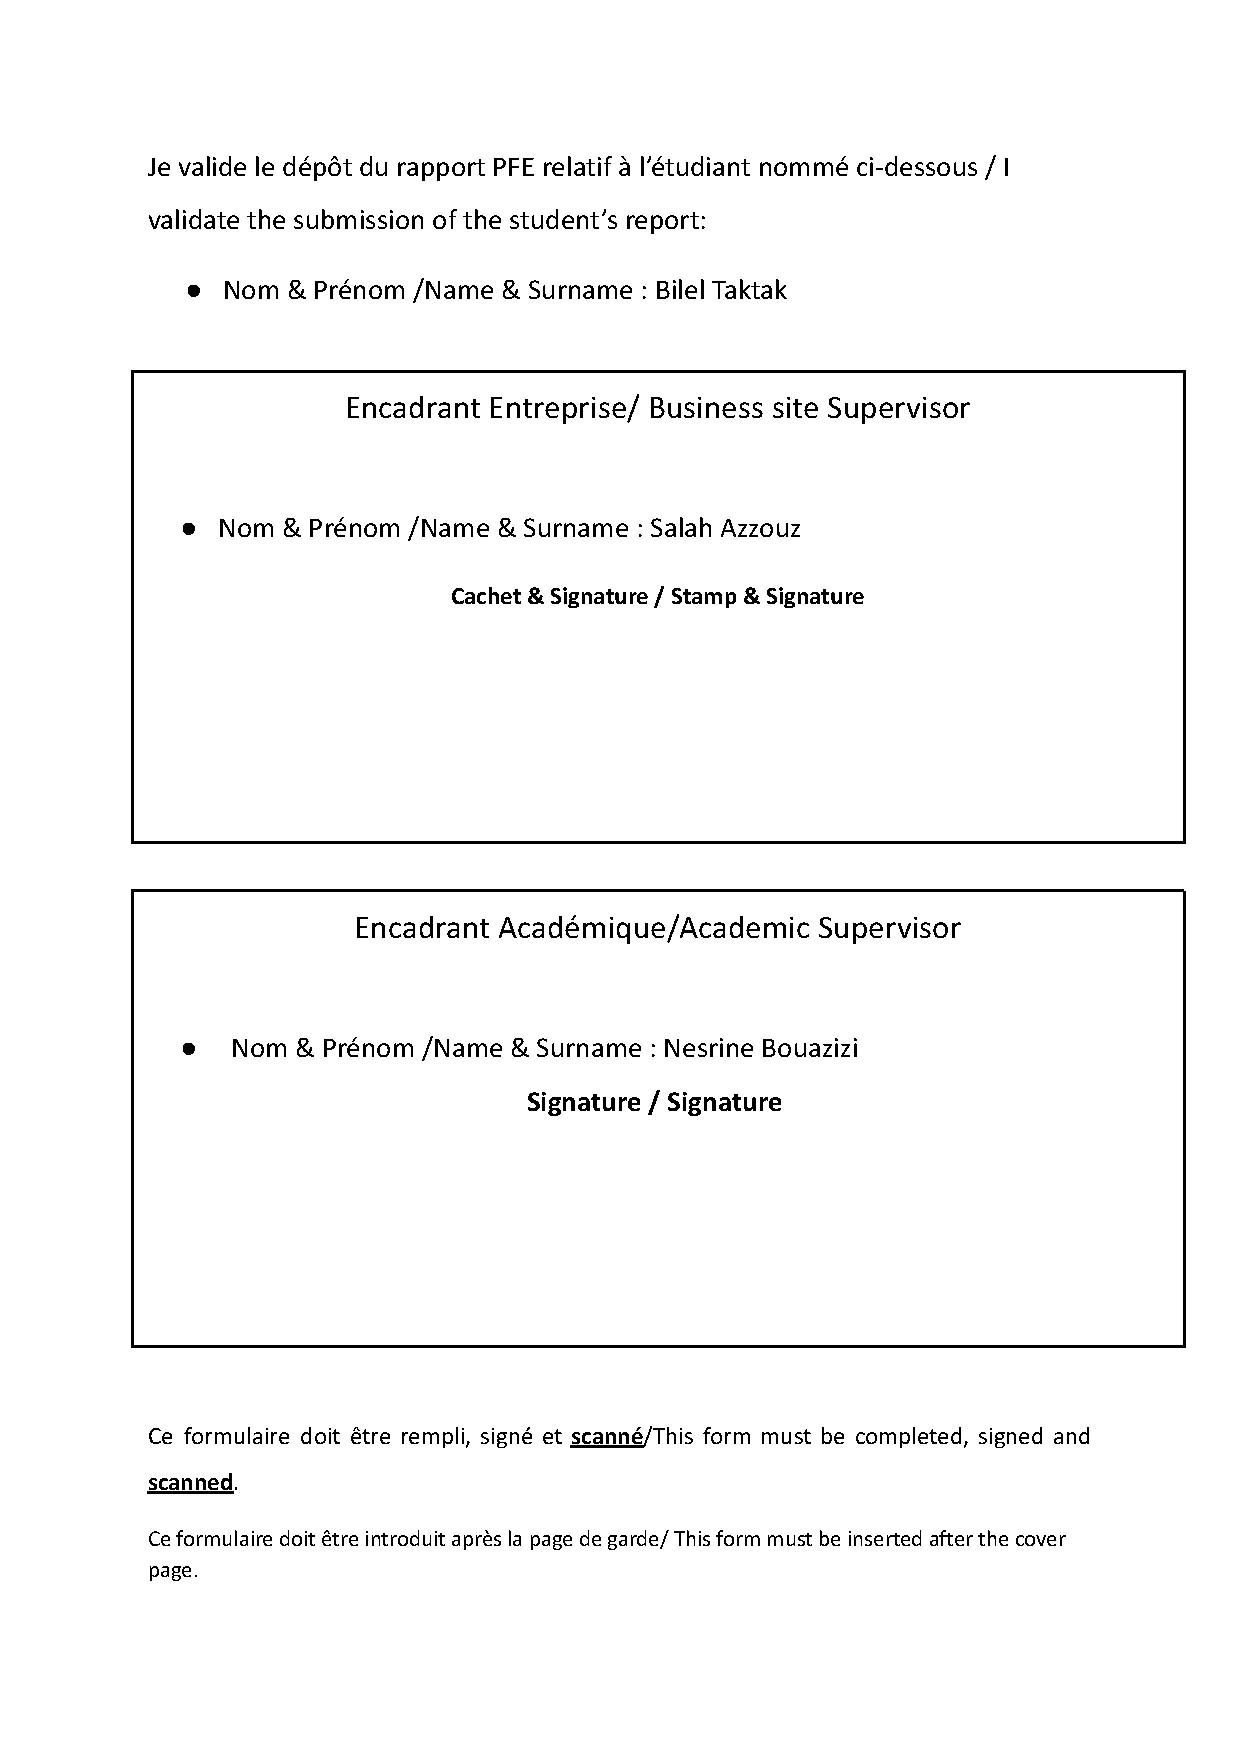
\includepdf[pages=1, fitpaper=true]{pdf/Page_de_Garde_Ang_split_1.pdf}
\cleardoublepage
\pagenumbering{gobble}
{
  \hypersetup{linkcolor=black}
  \tableofcontents
}
\cleardoublepage
\pagenumbering{arabic}
\cleardoublepage
\pagenumbering{gobble}
{
  \hypersetup{linkcolor=black}
  \listoffigures
}
\cleardoublepage
\pagenumbering{arabic}
\pagenumbering{gobble}
\clearpage
{
  \hypersetup{linkcolor=black}
  \listoftables
}
\clearpage
\pagenumbering{arabic}
\pagenumbering{gobble}
\clearpage
{
  \hypersetup{linkcolor=black}
  \printglossary[type=\acronymtype, title=List of Acronyms]
}
\clearpage
\pagenumbering{arabic}
\subfile{sections/Acknowledgement}
\subfile{sections/Introduction Generale}

\subfile{chapters/0 Cadre general}
\subfile{chapters/1 Approche}
\subfile{chapters/2 Exigences}
\subfile{chapters/3 Sprint 1.tex}
\subfile{chapters/4 Sprint 2.tex}
\subfile{chapters/5 Sprint 3.tex}

\subfile{sections/General Conclusion}

\cleardoublepage
\pagenumbering{gobble}
\printbibliography
\cleardoublepage
\pagenumbering{arabic}
\clearpage\thispagestyle{empty}\addtocounter{page}{-1} 

\includepdf[pages=1, fitpaper=true]{pdf/Page_de_Garde_Ang_split_2.pdf}
\end{document}
